\documentclass[12pt]{article}
\usepackage[T1]{fontenc}
\usepackage{graphicx}
\graphicspath{ {./} }

\author{
	Dominik Brdar \\
	bacc.ing.rac. Fakultet elektrotehnike i računarstva \\
	dominik.brdar@fer.hr
	\and
	Matija Holik \\
	bacc.ing.rac. Fakultet elektrotehnike i računarstva \\
	matija.holik@fer.hr
	\and
	Ivan Žugaj \\
	bacc.ing.rac. Fakultet elektrotehnike i računarstva \\
	ivan.zugaj@fer.hr
}



\begin{document}
	\begin{titlepage}
	\title{
		Simulacija života umjetnih organizama uz CUDA
	}
	\maketitle
	\end{titlepage}

	\section{Uvod}
	Izvođenje složenih izračuna s velikim brojem podataka kao što je simulacija međudjelovanja 
	populacija mikroorganizama različitih svojstava zahtjeva iznimno puno računalnih resursa.
	Grafička procesorska jedinica zbog svojstvene sklopovske arhitekture, koja omogućuje paralelno računanje 
	složenih operacija nad velikim skupom podataka, može se koristiti u svrhu ubrzavanja izvođenja procesa 
	takvih zadataka. Za programiranje grafičke kartice s ciljem kvalitetnije simulacije interakcija organizama 
	u sklopu ovog seminara, odabrana je CUDA platforma.
	
	Uz pomoć CUDA-e ćemo simulirati suživot organizama u tekućini s Ph vrijednošću jednakoj određenom broju različitih tipova organizma.
	
	Key words: simulation, parallelism, CUDA, CPU, arrays, PyCuda, PyCharm
	
	\section{Motivacija}
Jedna od klasičnih prikaza molekula i mikroorganizama je prikaz računalnom simulacijom. 
	Proučavanje i liječenje bolesti
za koje nije dovoljno promatrati živote organizama uz pomoć mikroskopa 
	ne bi bilo moguće bez takvih simulacija.
Mnoge tvrtke, poduzeća i istraživački centri značajno
doprinose 
	razvoju i kvaliteti lijekova koristeći računalne simulacije. 
	Kretanje i ponašanje velikog broja molekula i organizama iziskuje značajnu računalnu moć budući da 
	je potrebno obrađivati stotine tisuća objekata koji
se prikazuju u simulaciji. Osim njihovog postojanja,
	simuliraju se i brojene interakcije između samih organizama ili molekula. U takvom sustavu, elementi imaju 
	lokalne međuovisnosti, ali i neke globalne uvijete, te se za ovakve zadatke prikazuje da korištenje grafičke
	procesorske jedinice može znatno ubrzati proces simulacije. Nvidia CUDA (Compute Unified Device Architecture) nudi pristupačno programsko okruženje 
	za programiranje i korištenje grafičke kartice i njenog sklopovlja za paralelizaciju neovisnih računanja 
	i obradu velikog skupa podataka istovremeno. Proizvođač Nvidia, koji je sam i razvijao svoje grafičke kartice, 
	njihovu arhitekturu i programe na najnižoj razini, najbolje može ostvariti i programsku potporu pomoću koje 
	korisnici njihovih grafičkih kartica mogu svoje programe optimirati tako da za ključne dijelove implementiraju
	izvođenje na grafičkoj procesnoj jedinici. Na taj način, programer ne treba razumjeti svoju grafičku karticu 
	na niskoj razini, već koristi CUDA okruženje koje jamči najbolje iskorištavanje dostupnih resursa. S druge strane,
	takvi programi su optimirani samo za korisnike Nvidia grafičkih kartica, dok grafičke kartice drugih proizvođača
	imaju drugačija arhitekturna rješenja i neće moći interpretirati kod pisan pomoću CUDA platforme. Iako je 
	prenosivost mana, CUDA je ipak vrlo zastupljena u raznim područjima interesa kao što je strojno učenje ili block-chain
	tehnologije zbog nenadmašive preciznosti u smislu apsolutnog i optimalnog iskorištavanja grafičke kartice. 
		
	
	\section{Cilj rada}
	Produkt ovog rada je simulacija suživota 4 vrste istog zamišljenog organizma nazvanog Quid na određenoj površini unutar vode 
	pri neutralnoj pH vrijednosti (7).
Aktivnost tih organizama mijenja pH vrijednosti tekućine, a uz to se organizmi 
	unutar promatranog područja gibaju, rastu i među njima se događaju razne interakcije koje dovode do promijena 
	njihovih stanja. Za potrebe ilustracije učinkovitosti različitih programskih rješenja prikazana je i razlika izvršavanja simulacije korištenjem samo procesora i radne memorije, te uz pomoć grafičke kartice.
Pritom je cilj rada dobiti uvid
	u mogućnosti programiranja grafičke kartice za razne primjene, a ne samo za iscrtavanje. Ideja je da konačan ishod rada
	bude dodatna motivacija za nastavak proučavanja i uvođenja paralelizma u razne procese. 
	
	\section{Opis programskog rješenja}
	Prije početka simulacije korisnik odabire broj iteracija koje će se izvesti i koliko maksimalno quidova simulacija može generirati prije završetka.
	Potom odabire za svaku vrstu quidova koliko će ih se generirati na početku, veličinu područja koje se promatra i početnu temperaturu koja utječe na gibanje quidova u tom podučju.
	Nakon unosa parametara pokreće se simulacija.\\
	Korisnik ima mogućnost i centriranja canvasa kako bi simulacija bila na sredini prozora.
	Svaki od quidova tijekom simulacije kreće se 
	u različitim smjerovima koje su nasumične u x i y osi ovisno o incijalno postavljenoj temperaturi sustava čime dobivamo kaotičnost sustava. Na kraju svake iteracije Quidovi rastu za 1 te pri veličini od 8 dolazi do mejoze u kojem nastaju dva Quida, roditelj i dijete.
\\
	
	QUID
- Quidovi su podjeljeni na 4 različita tipa:
	\begin{enumerate}
		\item tip je crvene boje sa pH vrijednošću 3. 
		\item tip je žute boje sa pH vrijednošću 5.
		\item tip je zelene boje sa pH vrijednošću 9.
		\item tip je plave boje sa pH vrijednošću 12.
	\end{enumerate}
	Interakcije između različitih tipova opisane su u tablici \ref{tab:firstTable}.\\
	Vrste intekcija: X (množe se), - (ubiju se), 0 (nema učinka).
	Tipovi quidova se prikazuju brojevima (1, 2, 3, 4)\\
	\begin{table}[ht]
		\centering
		\begin{tabular}{|ccccc|}
			- & 1 & 2 & 3 & 4 \\
			1 & x & - & 0 & - \\
			2 & - & x & - & 0 \\
			3 & 0 & - & x & - \\
			4 & - & 0 & - & x \\
		\end{tabular}
		\caption{primjer matrice interakcija}
		\label{tab:firstTable}
	\end{table}
	\subsection{Tijek simulacije}
	Na ekranu se pojavljuje simulacija uz mogućnosti pauziranja, prekida simulacije i mogućnosti mijenjanja perioda svake iteracije radi lakšeg praćenja
	promijena i temperature u našem sustavu.\\
	Ispisuje se broj Quidova u simulaciji, kao i pH svakog kvadranta i cijelog sustava. Slika 3.1 prikazuje simulaciju u trenutku izvođenja.\\
	
	Simulacija se prekida u nekoliko slučajeva:
	\begin{itemize}
		\item kraj broja iteracija koje smo unijeli,
		\item nepostojanje quidova unutar simulacije budući da se quidovi kreću te prilikom izlaska izvan područja promatranja prestanu postojati,
		\item prekoračenje makismalnog broja quidova koje smo unijeli.
	\end{itemize}
	
	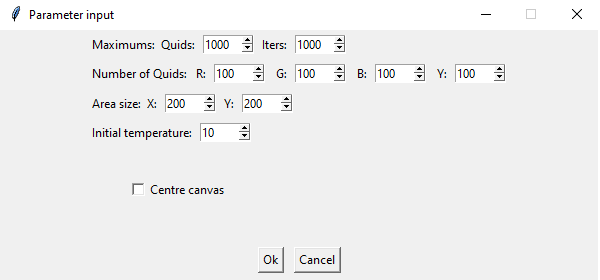
\includegraphics[scale=0.75]{parametri.png}
	
	
	
	\subsection{Promjene stanja quidova i izračun pH vrijednosti}
	Reakcija quidova događa se ovisno o njihovim tipovima kao što prikazuje tablica \ref{tab:firstTable}. Quidovi međusobno moraju biti na udaljenosti manjoj od 5 kako bi se interackija između njih dogodila.\\
	U rješavanju programskog dijela dolazilo je do više problema. Budući da pyCuda u većini slučajeva radi sa matricama, kretanje svake jedinke Quida dostavljeno je u matrici sa svojom trenutačnom pozicijom te bi CUDA potom odradila izračun kretanja svakog Quida čime bi se ona kretala u x i y smjeru prema svom vektoru smjera.
	Zbog strukture podataka dolazilo je do problema pri konverziji iz GPU kompatibilne strukture podataka u podržani matrični oblik. 
	Rješavanje izračuna udaljenosti bi se izvodio također matrično gdje bi u prvom retku matrice  i u prvom stupcu bio prvi Quid koji bi potom imao vrijednosti udaljenosti svih svojih susjeda. \\
	Drugi Quid bi bio u drugom retku u prvom stupcu te bi izračunao udaljenosti svakog Quida od svakog i tako bi dobili matricu veličine $\mathbf{N^2}$.
	Nakon izračuna bi svaki Quid obavio interakciju sa svojim najbližim susjednom i dobio postavljenu zastavicu za obavljenu interakciju.
	
	\includegraphics[scale=0.45]{simulacija.png}
	
	\section{Osvrt na rezultat}
	U radu sa sučeljem vezano za GPU korišten su alati PyCuda i Cupy, no alati nemaju transparentnu vezu stoga je međukomunikacija zahtijevala temeljnije poznavanje alata i pripadnih podatkovnih struktura. U main.py opisana je simulacija klasično sekvencijske izvedbe programa, dok u main2.py uvedena osnovna upotreba vektorskog računanja pomoću CPU čime je performasna uvelike ubrzana. U main3.py i main4.py uvedeni su pokušaji izvedbe simulacije preko GPU korištenjem alata PyCuda i Cupy koji zbog unutarnjih nekonzistentnosti strukture podataka nisu uspjeli postići funkcionalnost izvedenu u main2.py. 
	
	\section{Zaključak}
	Simulacija umjetnih i realnih molekula ili mikroorganizama jedno je od kompleksnim područja zbog svog iznimno velikog 
    broja jediniki i prikaza njihovih ponašanja kako bismo ih što bolje prikazali u svojoj prirodi. Znanstvenici uz pomoć
    modernih alata poput CUDA i sličnih alata olakšavaju izračune preko kojih prikazuju ove pojave. Korištenjem CPU i RAM-a 
    naspram korištenjem GPU-a rezultira dužim periodom izvršavanja čime ne bismo uštedjeli vrijeme zbog nemogućnosti CPU za izvršavanje velikog broja paralelnih vektorskih operacija.
    Za razliku od toga korištenjem CUDA iskorištavamo masovne paralelne mogućnosti GPU čime dolazi do dodatnog mjesta za napredak izvođenja simulacije sa
    potencijalnom novim parametrima.
    
\end{document}
